\section{Intro}
\todo[inline, author=Jens]{Why is this subject important?
What can we use it for?
Who is it interesting for?
Background}

To realize the vision of continuously expanding human abilities in robotics surely the visual system is of great importance and specifically the task of object recognition is essential to the humanoid robot.

The primate brain's ability to categorize and recognize objects could lead to the idea that the task in its general sense is easy and therefore also easily copied onto an artificial system ie. “Computer vision”. However it is not.
Although the idea of implementing a visual computer system analogue to the biological visual system in the primate brain has existed since the 1970's there is still long way for such a system to be developed. The theories proposed by neuroscientist David Marr \citep{VisualHierarchy} had, until recently been found difficult to implement due to lack of computational power. Hence the main focus in general computer vision has been on designing individual task oriented algorithms that perform analysis and recognition of such features as color shape etc.
The specific task of object recognition through pixel-information might seem easy as the human brain seems to do it instantly and effortlessly. However the seemingly unlimited amount of different objects in addition to variation of size, and posture in the 3D space is a great obstacle in the development of object recognition. Imaging a the simple concept of a cup. As humans we instantly recognize the use of it even when we have never seen that specific type of cup. Size, shape, handle, no handle colour etc.


\section*{Flat processing Schemes vs. Deep Hierarchies}
In the SIFT structure an object is identified by obtaining features, known as keys, in an input image and then search for these features in a database. When multiple statements point at a specific object further effort will be made to specify it. The complexity of this unbounded visual search(refereed to as flat processing scheme) is NP complete\citep{fidler2009learning}.

\begin{figure}[h!] %fancyboxes
\centering
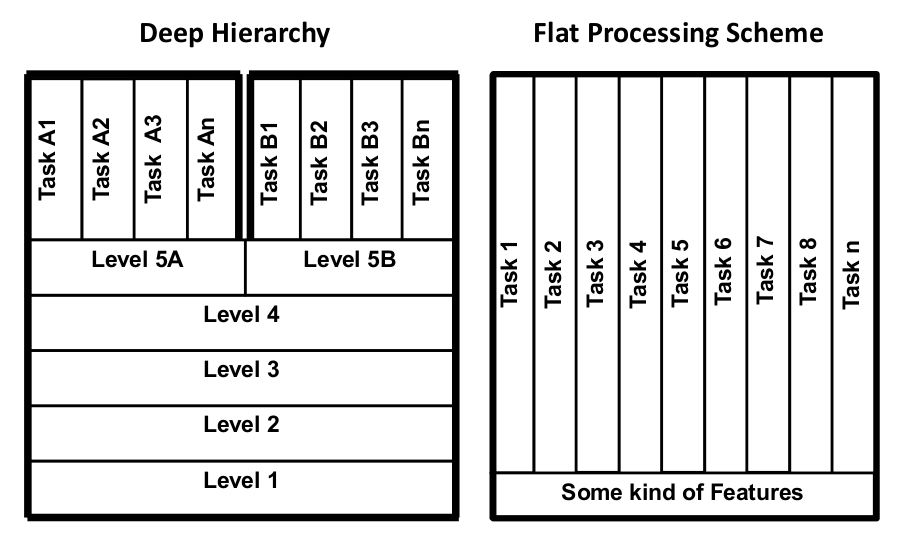
\includegraphics[width=0.5\textwidth]{graphics/deepvsflat}
\caption{Deep hierarchies and flat processing schemes}
\label{fig:deepvsflat}
\end{figure}

A solution build on a hierarchal structure could very well be the best way to develop such a system as it has been found in the primate brain. As mentioned the human brain seem to interpret visual stimuli with very little effort and therefore trying to emulate the brain of primates might help in optimizing object recognition in computer vision. Especially the relatively recent development of multi-core systems in computer science greatly supports the development of these structures as parallel processing is of fundamental character in the primate brain.\citep{fidler2009learning}  \\
A hierarchical model consists of a number of layers placed “on top of each-other”. Each item in a layer, representing more advanced features, is composed of items from the layers below which represents simpler features. The smallest feature being an edge. 
(Based on Visual Hierachies)
This form of representation gives some main advantages taking the aspect of computational efficiency and storage space into account. As said before layers of more advanced features are composed from elements of the layer below hence only the fundamental building blocks are stored along with information regarding connections of compositions. In addition this method takes advantage of the fact that some lower level items will be reused in many of the items in layers above which minimizes the need of duplicates. With this form of representation we only need very few actual descriptors around 10-20 in the lower layers and in the range of thousands in the upper layers\citep{fidler2009learning}. 
In fact the best “flat processing schemes” of today must store millions of small images with 25 x 25 pixels as descriptors in order to get satisfying results which is in great contrast to hierarchies.\citep{fidler2009learning}

Another advantage of the Deep Hierarchy is what is refereed to as generalization. Generalization means that like in the primal brain we can make common calculations that will apply for several individual tasks related to computervision such as object recognition and categorization, grasping, manipulation, path planning, etc. \textbf{(REF:Visual Hierarchies)}